\section{Auswertung}
\label{sec:Auswertung}

\subsection{Vorbereitung}
\subsubsection{Vorbereitungsaufgaben}

Als Vorbereitung auf die Versuchsreihe, werden Literaturwerte zur Dichte und Schallgeschwindigkeit verschiedener
Materialien recherchiert. Anschließend wird die Impedanz mithilfe von $Z = \rho \cdot c$ ausgerechnet.\\
Die Werte lassen sich in \autoref{tab:Literaturwerte} finden.
\begin{table}
  \centering
  \caption{Literaturwerte und akustische Impedanzen verschiedener Materialien.}
  \label{tab:Literaturwerte}
  \begin{tabular}{c | l l l}
    Material & Schallgeschwindigkeit $c$ / $\frac{\mathrm{m}}{\mathrm{s}}$ & Dichte $\rho$ / $\frac{\mathrm{g}}{\mathrm{cm}^3}$ & Akustische Impendanz $Z$ / $\frac{\mathrm{kg}}{\mathrm{sm}^2} \cdot 10^6$\\
       \midrule
        Luft    & 331 \cite{medizinphysik}     & 1,300 $\cdot 10^{-3}$ \cite{medizinphysik}& 4,3 $\cdot 10^{-4}$ \\
        Wasser  & 1492 \cite{medizinphysik}    & 0,9982 \cite{medizinphysik}               & 1,48 \\
        Blut    & 1530 \cite{medizinphysik}    & 1,03   \cite{medizinphysik}               & 1,56  \\
        Knochen & 3600 \cite{medizinphysik}    & 1,7    \cite{medizinphysik}               & 6,12  \\
        Acryl   & 2730 \cite{thiemann}        & 1,189  \cite{imeter}                       & 3,25  \\
      \bottomrule
    \end{tabular}
\end{table}
Anschließend wird die Wellenlänge und die Periode einer 2 MHz Schwingung in Acryl ausgerechnet.
\begin{align}
  \label{eqn:lambdaacry}
  \lambda = \frac{c}{f} = 1,365 \cdot 10^{-3} \, \mathrm{m} \\
  \label{eqn:Tacry}
  T = \frac{1}{f} = 0,5 \cdot 10^{-6} \, \mathrm{s}
\end{align}

\subsubsection{Kennenlernen und Einstellen des Programms}

Mit der Schieblehre wird die Dicke der ausgewählten Acrylplatte gemessen. Diese beträgt $d=(9,95 \pm 0,05) \, \cdot 10^{-3} \, \mathrm{m}$.\\
Anschließend wird ein A-Scan durchgeführt, welcher die Graphik in \autoref{fig:1cmAcrylplatt} erzeugt.\\
\begin{figure}
  \centering
  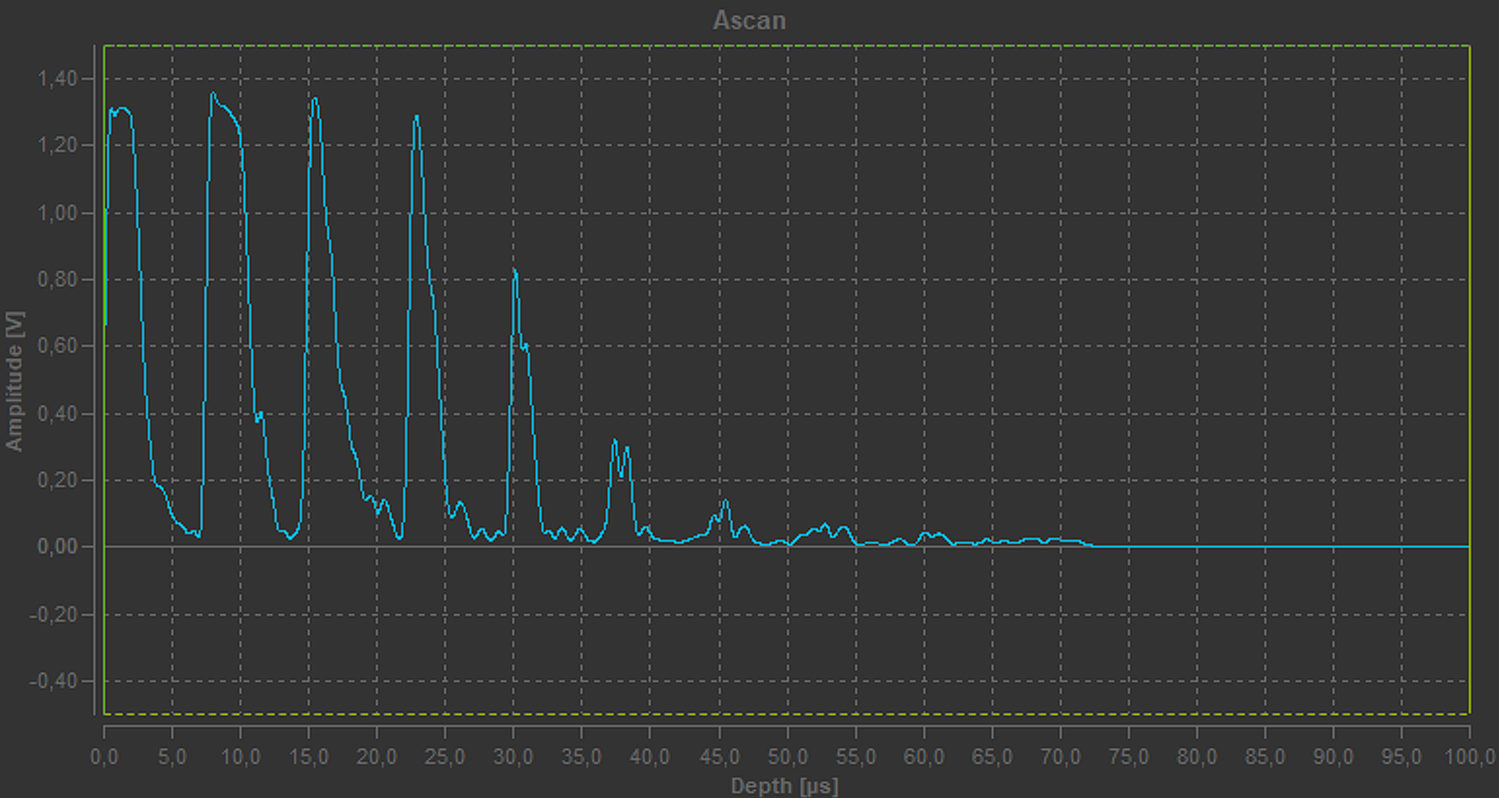
\includegraphics[width=15cm]{messwerte/Vorbereitung/AScan_Vorbereitung.png}
  \caption{A-Scan der 1 cm dicken Acrylplatte.}
  \label{fig:1cmAcrylplatt}
\end{figure}
In der Abbildung lassen sich fünf Schwingungen besonders gut erkennen. Von diesen Schwingungen wird die Laufzeit und
Amplitude mittels importierter Daten aus dem Programm bestimmt und in \autoref{tab:LaufzeitenUndAmplituden} aufgelistet.
\begin{table}
  \centering
  \caption{Laufzeiten und Amplituden der ersten fünf Schwingungen.}
  \label{tab:LaufzeitenUndAmplituden}
  \begin{tabular}{c | c c}
    Schwingung & Laufzeit $t$ / $\si{\micro\second}$ & Amplitude $A$ / $\si{\volt}$ \\
       \midrule
        1 & 7,12  & 1,316 \\
        2 & 7,28  & 1,366 \\
        3 & 7,40  & 1,340 \\
        4 & 7,64  & 1,297 \\
        5 & 7,22  & 0,880 \\
      \bottomrule
    \end{tabular}
\end{table}
Aus den gemessenen Daten wird der Mittelwert der Laufzeit und anschließend die Schallgeschwindigkeit mittels \autoref{eqn:Strecke} bestimmt.\\
Mittelwert der Laufzeit:
\begin{align*}
  t &= (7,33 \pm 0,09) \, \si{\micro\second} \\
  c &= \frac{2s}{t} \\
  c &= (2714,87 \pm 13,64) \, \si{\meter\per\second}
\end{align*}
Die Unsicherheit wurde mittels Gaußscher Fehlerfortpflanzung bestimmt. Die Schallgeschwindigkeit in Acryl lautet somit
$c_{\mathrm{Acryl}} = (2714,87 \pm 13,64) \, \si{\meter\per\second}$.\\
Nun wird zwischen den Anzeigemodi $AM$, $HF$ und $AM + HF$ gewechselt und Bilder der Modi aufgezeichnet. Die Bilder sind 
in \autoref{Modi} gezeigt.
\begin{figure}
	\centering
	\begin{subfigure}[b]{0.3\textwidth}
		\centering
		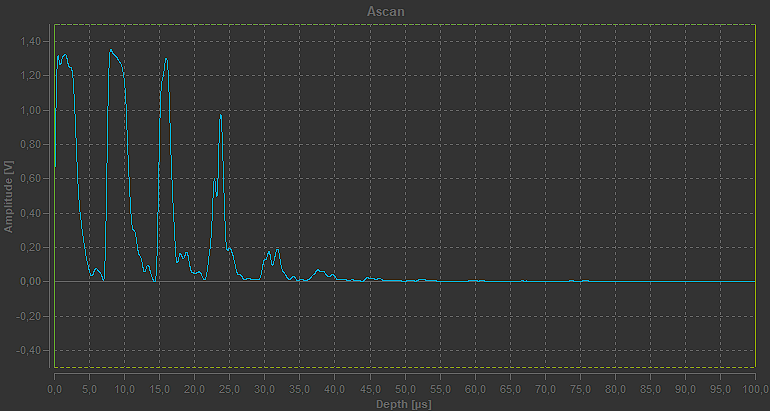
\includegraphics[width=4.5cm]{messwerte/Vorbereitung/Amp.png}
		\caption{$AM$ Modus}
	\end{subfigure}
	~
	\begin{subfigure}[b]{0.3\textwidth}
		\centering
		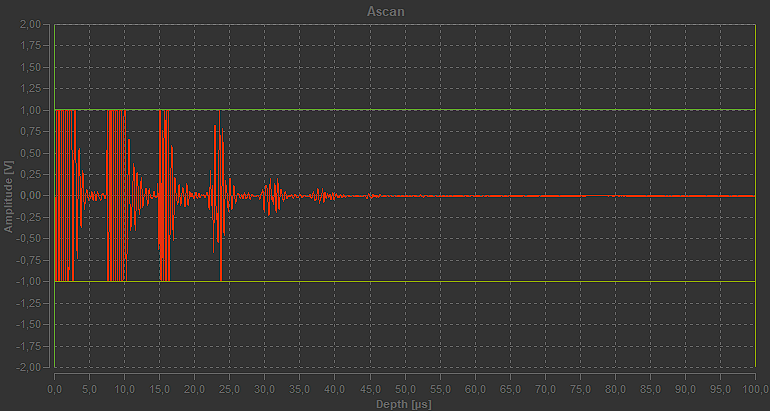
\includegraphics[width=4.5cm]{messwerte/Vorbereitung/HF.png}
		\caption{$HF$ Modus}
	\end{subfigure}
	~
	\begin{subfigure}[b]{0.3\textwidth}
		\centering
		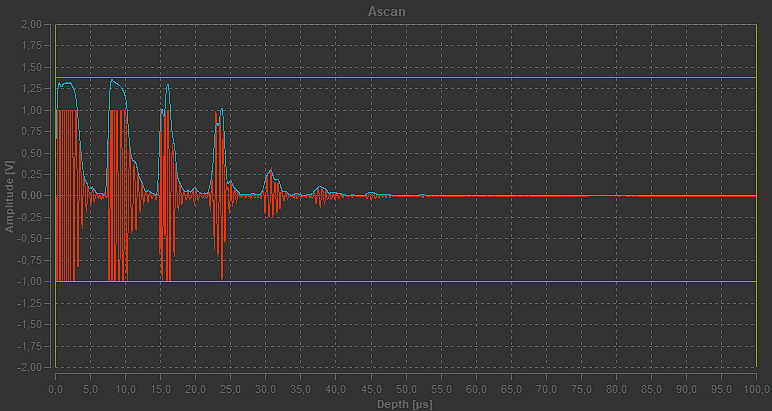
\includegraphics[width=4.5cm]{messwerte/Vorbereitung/HF+Amp.png}
		\caption{$AM + HF$ Modus}
	\end{subfigure}
  \caption{Alle drei verschiedenen Anzeigemodi}
  \label{Modi}
\end{figure}

Es lässt sich erkennen, dass im $HF$-Modus jede einzelne Schwingung angezeigt wird, während
im $AM$-Modus jeweils nur die positiven Amplituden jener Schwingungen angezeigt werden. Im $AM + HF$-Modus
werden jene zwei Modi kombiniert ausgegeben.\\
Je nach Versuchsteil wird ein anderer Modus verwendet.\\
Als nächstes wird der $AM + HF$-Modus eingeschaltet und bei einer 2 MHz Schwingung die Periode einer Schwingung
ausgerechnet. Dafür wird über fünf Perioden hinweg gemittelt. Der verwendete Bereich ist mittels grünen Balken 
in \autoref{fig:T} eingezeichnet.
\begin{figure}
  \centering
  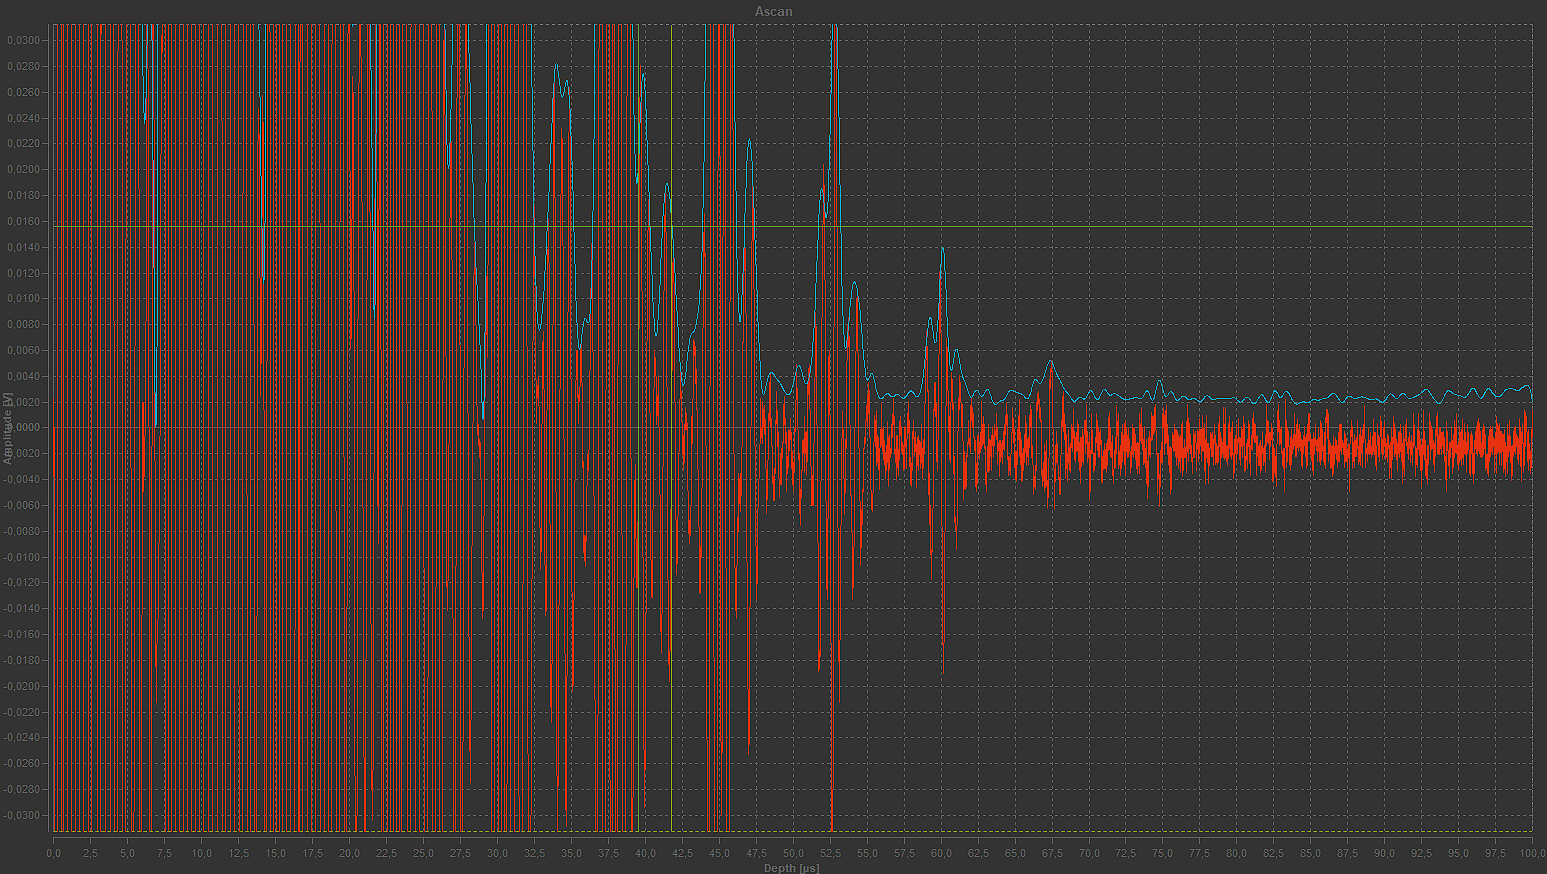
\includegraphics[width=15cm]{messwerte/Vorbereitung/T.png}
  \caption{2 MHz Schwingung im $AM + HF$-Modus angezeigt.}
  \label{fig:T}
\end{figure}
Die fünf Perioden zusammenaddiert haben eine Länge von $T_5 =2,2 \, \si{\micro\second}$. Dieser Messwert wird
durch fünf geteilt, um die Länge einer Periode zu erhalten: $T_1 = \frac{2,2}{5} \, \si{\micro\second} = 0,44 \, \si{\micro\second}$.
Daraus lässt sich nun die Wellenlänge und Frequenz der Schwinung in Acryl berechnen:
\begin{align*}
  f &= \frac{1}{T} = 2 272 727,27 \, \si{\per\second} = 2,3 \, \mathrm{MHz}\\
  \lambda &= (1,19 \pm 0,01) \cdot 10^{-3} \, \si{\meter}
\end{align*}
Mittels der Tiefenmessung des Programms wird für die Acrylplatte eine Dicke von 1 cm gemessen.

\subsection{Ausmessen der verwendeten Acrylzylinder}

Insgesamt stehen vier verschiedene Größen von Acrylzylindern zur Verfügung. Diese werden alle mit einer Schieblehre
ausgemessen. Die Messwerte sind in \autoref{tab:Zylinder} eingetragen. Die Schieblehre hat eine Messungenauigkeit von
0,05 mm.

\begin{table}
  \centering
  \caption{Messwerte der vier verschiedenen Acrylzylinder.}
  \label{tab:Zylinder}
  \begin{tabular}{c | c c}
    Zylindernummer & Höhe $h$ / $\si{\milli\meter}$ & Durchmesser $d$ / $\si{\milli\meter}$ \\
       \midrule
        1 & 120,90 & 40,00 \\
        2 & 80,50  & 40,10 \\
        3 & 61,55  & 40,45 \\
        4 & 40,45  & 40,15 \\
      \bottomrule
    \end{tabular}
\end{table}

\subsection{Schallgeschwindigkeitsbestimmung mit dem Impuls-Echo-Verfahren}

In dieser Versuchsreihe werden die vier Zylinder mittels Impuls-Echo-Verfahren beschallt. Zudem wird noch
ein 10 cm großer Zylinder aus den einzelnen Zylindern gebaut und beschallt.

\begin{table}
  \centering
  \caption{Zur Bestimmung der Schallgeschwindigkeit mit Impuls-Echo-Verfahren aufgenommene Messwerte.}
  \label{tab:EchoImpuls}
  \begin{tabular}{c | c c c c}
    Höhe $h$ / $\si{\milli\meter}$ & Ausges. Imp. $U_A$ / $\si{\volt}$ &  Startzeit $t_0$ / $\si{\micro\second}$ & Refklekt. Imp. $U_R$ / $\si{\volt}$ & Endzeit $t_R$ / $\si{\micro\second}$ \\
       \midrule
        40,45 & 1,318 & 1,260 & 1,250 & 30,26 \\
        61,55 & 1,318 & 1,280 & 0,619 & 46,04 \\
        80,50 & 1,319 & 1,240 & 0,304 & 59,50 \\
        102,00 & 1,318 & 1,260 & 0,068 & 75,34 \\
        120,90 & 1,319 & 1,260 & 1,193 & 88,56 \\
      \bottomrule
    \end{tabular}
\end{table}

Mittels dieser Messwerte wird eine lineare Ausgleichsrechnung mit Python durchgeführt. Die Theoriekurve ergibt sich aus
\autoref{eqn:Strecke} und einer Anpassungsschicht $d$ für die Sonde. Die Geradengleichung lautet also
\begin{equation}
  2l = c \cdot t + d.
\end{equation}
$l$ ist die jeweilige Länge des Zylinders und $t = t_R - t_0$ die Laufzeit der Schwingung. $t_0$ ist der Zeitpunkt
des Peaks des ausgesendeten Impulses und $t_r$ der Zeitpunkt des Peaks des reflektierten Impulses.\\
Mittels Python ergibt sich dann die Steigung und der y-Achsenabschnitt der Geraden. Die Steigung entspricht
der Schallgeschwindigkeit in Acryl $c_{\mathrm{Acryl}}$ und der y-Achsenabschnitt entspricht der Anpassungsschicht $d$.\\
\begin{align*}
  c_{\mathrm{Acryl}} &= (2,75895 \pm 0,01631) \, \si{\milli\meter\per\micro\second} &= (2758,95 \pm 16,31) \, \si{\meter\per\second} \\
  d &= (0,26 \pm 1,02) \, \si{\milli\meter} &= (0,26 \pm 1,02) \cdot 10^{-3} \, \si{\meter}
\end{align*}
Die Messwerte und Ausgleichsfunktion sind in \autoref{fig:ImpulsEcho} dargestellt.
\begin{figure}
  \centering
  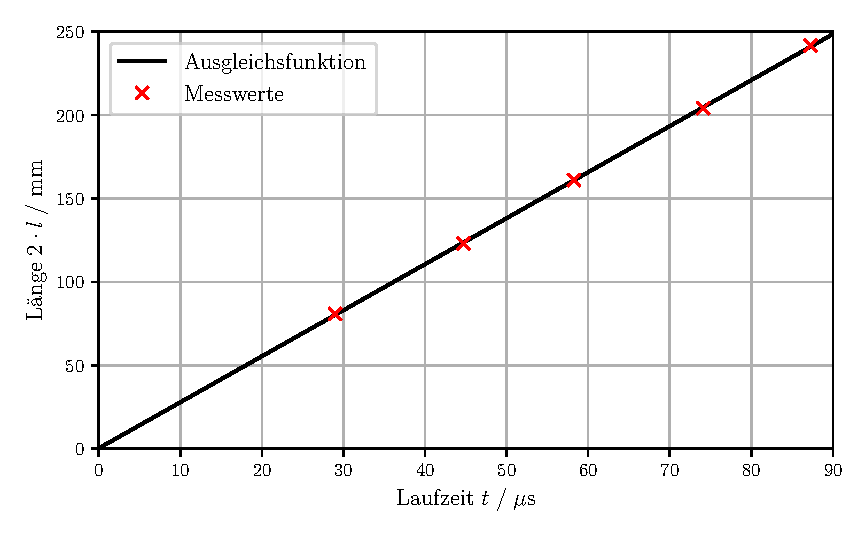
\includegraphics[width=15cm]{messwerte/ImpulsEcho.pdf}
  \caption{doppelte Zylinderhöhe $l$ geplottet gegen die Laufzeit $t$ beim Impuls-Echo-Verfahren.}
  \label{fig:ImpulsEcho}
\end{figure}

\subsection{Schallgeschwindigkeitsbestimmung mit Durchschallungs-Verfahren}

Für diese Versuchsreihe werden alle 4 Zylindergrößen horizontal platziert und mittels zwei Sonden durchschallt.\\
Mit diesem Verfahren ergibt sich für die Strecke die Gleichung 
\begin{equation}
  l = c \cdot t + d,
\end{equation}
da der Weg bis zur Singnalempfangung nur einmal zurückgelegt wird.\\
Mittels A-Scan wird die Laufzeit des Impulses gemessen und in %\auotref{tab:Durchschallung} aufgelistet.
\begin{table}
  \centering
  \caption{Zur Bestimmung der Schallgeschwindigkeit mit Durchschallungs-Verfahren aufgenommene Messwerte.}
  \label{tab:Durchschallung}
  \begin{tabular}{c | c c}
    Höhe $h$ / $\si{\milli\meter}$ & Zeitpunkt eingehender Impuls $t_0$ / $\si{\micro\second}$ & Zeitpunkt reflektierter Impuls $t_R$ / $\si{\micro\second}$ \\
       \midrule
         40   & & \\
         60   & & \\
         80   & & \\
         120  & & \\
      \bottomrule
    \end{tabular}
\end{table}


\subsection{Bestimmung der Dämpfung mit dem Impuls-Echo-Verfahren}

\subsection{Biometrische Untersuchung eines Augenmodells}